% Main dissertation file
\documentclass[12pt,a4paper,oneside]{report}

% ---- Packages ----
\usepackage[utf8]{inputenc}
\usepackage[T1]{fontenc}
\usepackage{geometry}
\usepackage{setspace}
\usepackage{graphicx}
\usepackage{booktabs}
\usepackage{longtable}
\usepackage{array}
\usepackage{caption}
\usepackage{subcaption}
\usepackage{hyperref}
\usepackage{url}
\usepackage{amsmath}
\usepackage{amssymb}
\usepackage{siunitx}
\usepackage{listings}
\usepackage{xcolor}
\usepackage{float}
\usepackage{enumitem}
\usepackage{titlesec}
\usepackage{lmodern}
\usepackage{microtype}
\usepackage{tikz}
\usepackage{pgfplots}
\usetikzlibrary{arrows.meta,positioning,shapes.geometric}
\pgfplotsset{compat=1.18}

% ---- Page setup ----
\geometry{margin=1in}
\onehalfspacing
\hypersetup{
  colorlinks=true,
  linkcolor=black,
  urlcolor=blue,
  citecolor=black
}

% ---- Code style ----
\lstdefinestyle{codestyle}{
  basicstyle=\ttfamily\small,
  breaklines=true,
  frame=single,
  backgroundcolor=\color{gray!5},
  keywordstyle=\color{blue!60!black},
  commentstyle=\color{green!50!black},
  stringstyle=\color{orange!60!black}
}
\lstset{style=codestyle}

% ---- Diagram styles ----
\tikzset{
  block/.style={rectangle, draw, rounded corners, align=center, minimum width=2.7cm, minimum height=0.9cm},
  smallblock/.style={rectangle, draw, rounded corners, align=center, minimum width=2.3cm, minimum height=0.8cm},
  line/.style={-Latex, thick}
}

% ---- Title info ----
% ---- Heading sizes ----
% Title: 16pt, Section: 14pt, Subsection: 13.8pt, Subsubsection: 13.6pt
\titleformat{\chapter}
  {\normalfont\fontsize{16pt}{20pt}\bfseries}
  {\thechapter}{1em}{}
\titleformat{\section}
  {\normalfont\fontsize{14pt}{18pt}\bfseries}
  {\thesection}{1em}{}
\titleformat{\subsection}
  {\normalfont\fontsize{13.8pt}{17pt}\bfseries}
  {\thesubsection}{1em}{}
\titleformat{\subsubsection}
  {\normalfont\fontsize{13.6pt}{17pt}\bfseries}
  {\thesubsubsection}{1em}{}

% ---- Title info ----
\title{Predictive Analytics for Traffic Congestion in Urban Areas: A London Case Study}
\author{Narendra Chitirala}
\date{MSc Big Data Analytics}

\begin{document}

% ---- Front matter ----
\begin{titlepage}
  \centering
  {\fontsize{16pt}{20pt}\selectfont \textbf{Predictive Analytics for Traffic Congestion in Urban Areas: A London Case Study} \par}
  \vspace{1cm}
  {\large MSc Big Data Analytics \par}
  \vspace{1cm}
  {\large Author: Narendra Chitirala \par}
  \vspace{0.5cm}
  {\large Institution: Sheffield Hallam University \par}
  \vspace{0.5cm}
  {\large Submission Date: Jan 2026 \par}
  \vfill
  {\large Supervisor: Gregor Milligan \par}
\end{titlepage}

\pagenumbering{roman}

\chapter*{Abstract}
Outputs are visualized through dual dashboards: a web-based Mapbox interface hosted on GitHub Pages at \url{https://narendrachit.github.io/Traffic_prediction/} and a desktop Power BI dashboard.

\chapter*{Acknowledgements}
The author expresses sincere gratitude to Gregor Milligan for consistent guidance, constructive critique, and encouragement throughout the dissertation process. Appreciation is extended to academic staff in the MSc Big Data Analytics programme for the rigorous curriculum that underpinned the methodological and technical components of this work. Thanks are also offered to peers and colleagues who reviewed drafts, tested the pipeline, and shared practical advice on data engineering workflows. The support of family and friends is acknowledged for patience, motivation, and understanding during intensive stages of implementation and writing. Access to open data from the Department for Transport and Transport for London is gratefully recognized, as these sources made the empirical study possible. The project benefited from the open source community behind Apache Spark, Airflow, Mapbox, and related libraries, whose documentation and tooling enabled rapid development and reproducibility. Gratitude is also extended to classmates who shared seminar feedback and to the university ethics process that provided a clear framework for responsible data use. Institutional facilities, including computing resources and library access, provided an enabling environment for experimentation, literature review, and formal writing, and these contributions are acknowledged with gratitude. Administrative support during submission preparation is also appreciated for ensuring deadlines, formatting checks, and procedural requirements were met.

\tableofcontents
\listoffigures
\listoftables

\clearpage
\pagenumbering{arabic}

% ---- Chapters ----
\chapter{Introduction}
\section{Urban congestion context}
Urban traffic congestion is a persistent systems problem shaped by rapid urbanization, constrained road space, and complex travel demand. In large cities such as London, congestion affects travel time reliability, air quality, and the economic efficiency of freight and commuter mobility. The public sector and private operators face operational and strategic challenges that require data driven planning. Traditional traffic management relies on historical averages and manual reporting, which are insufficient for modern network complexity. The growing availability of open transport datasets creates an opportunity to move from descriptive reporting to predictive analytics. Forecasting congestion at an hourly resolution enables proactive interventions, targeted infrastructure investment, and scenario evaluation. The London road network provides a rich case study because it combines dense traffic, diverse road categories, and active policy initiatives focused on congestion reduction. The technical challenge lies not only in building a predictive model but in creating a repeatable data pipeline that can process large datasets, reconcile inconsistent inputs, and deliver outputs in a form that is accessible to decision makers.

Congestion is a multi dimensional phenomenon involving volume, speed, and variability. In the absence of direct travel time data, traffic volume serves as a robust proxy that correlates with delay on urban roads. This proxy allows the use of long term count datasets and supports large scale modeling. The complexity of traffic dynamics in London highlights the need for temporal features that capture periodic patterns, as well as external indicators such as disruptions that alter normal flow. The project therefore frames congestion prediction as a structured regression task with clearly defined inputs and outputs. The broader objective is to demonstrate that predictive analytics can be operationalized within a disciplined data engineering architecture, rather than remaining as isolated experiments. This framing aligns with the expectations of an MSc Big Data Analytics project where both analytical rigor and system design are assessed.

A further consideration is the policy context in which congestion analytics are used. Decisions on road pricing, signal timing, and maintenance schedules increasingly rely on evidence derived from data. A pipeline that provides consistent outputs enables comparisons across time and supports monitoring of policy interventions. The emphasis on hourly forecasting reflects the cadence of operational decision making, where short term predictions are more actionable than monthly aggregates. This context motivates a system that is both technically robust and operationally interpretable, ensuring that analytical outputs can be integrated into planning workflows.

\section{Motivation and practical drivers}
The motivation is both technical and applied. Technically, the project demonstrates an end to end data pipeline that integrates heterogeneous sources, handles large volumes of records, and produces machine learning outputs suitable for spatial analysis. Practically, the outcomes support two operational decisions: where congestion hotspots occur and how routing strategies can avoid them. Public sector agencies require evidence based insights rather than static dashboards. A reproducible pipeline reduces the cost of updates, supports auditability, and makes it possible to extend the system to new regions or alternative targets. The use of Apache Spark and Airflow reflects industry practice for reliable orchestration and scalable processing. A web based Mapbox dashboard translates analytical outputs into an interpretable geospatial product for users who are not data engineers. The combination of predictive modeling and routing analysis provides a coherent narrative from data ingestion to actionable insight.

The project also addresses a common gap in applied data science work: the transition from model outputs to operational decision support. Many academic studies report accuracy metrics without demonstrating how the predictions inform spatial planning or routing choices. In this work, predicted congestion is converted to hotspot rates at the road segment level and then used to weight a routing graph. This transformation provides a concrete example of how model outputs can be embedded into a downstream task. Another motivation is transparency. Open datasets and reproducible code allow the pipeline to be audited, which is particularly important in public policy contexts where transparency is essential. The project therefore emphasizes both the analytical pipeline and the governance of data processing.

A practical driver is the need to balance scalability with local execution. Many public sector projects operate with limited infrastructure and require solutions that can run on commodity hardware. The pipeline is designed to run in a local environment while adopting scalable patterns such as partitioned storage and containerized tasks. This provides a bridge between prototype and production and demonstrates how big data tooling can be used effectively in resource constrained settings.

\section{Research aim and objectives}
The aim of this dissertation is to design, implement, and evaluate a scalable pipeline for predicting urban traffic congestion and visualizing congestion aware routing outputs. The objectives are: (1) acquire and harmonize London traffic count data with disruption data, (2) engineer temporal and spatial features suitable for supervised learning, (3) train and evaluate forecasting models under walk forward validation, (4) generate spatial outputs that quantify hotspot risk by road segment, (5) implement a routing post processing stage that compares shortest distance and congestion aware routes, and (6) deliver a web based dashboard that communicates predictions and route comparisons. These objectives guide the chapter structure and the evaluation framework used throughout the report.

The contributions of this dissertation are:
\begin{itemize}[leftmargin=*]
  \item Reproducible pipeline (Airflow $\rightarrow$ Spark $\rightarrow$ curated datasets).
  \item Walk forward evaluation for robust temporal validation.
  \item Hotspot forecasting and spatial analytics for congestion risk.
  \item Dashboard for decision support with maps and route suggestions.
\end{itemize}

Each objective corresponds to a distinct technical deliverable. Data acquisition involves automated download and structured storage. Feature engineering requires conversion of raw timestamps and categorical data into numeric variables. Model training and evaluation involve configuring Spark ML pipelines and selecting metrics appropriate for time series forecasting. Spatial outputs require a transformation from tabular predictions to GeoJSON, which requires a routing graph and coordinate mapping. The dashboard integrates these outputs into an interactive map that supports filtering and comparison. The objectives are designed to ensure that the final outcome is not only a predictive model but also a complete analytics system that can be executed end to end.

The objectives also provide clear checkpoints for validation. Data integration can be validated by inspecting cleaned parquet outputs. Feature engineering can be validated through schema checks and summary statistics. Model training is validated using evaluation metrics and visual inspection of residuals. Spatial outputs are validated through map overlays and route statistics. These checkpoints ensure that progress can be measured objectively throughout the project.

\section{Research questions}
Four research questions structure the work. RQ1 (Forecasting): How accurately can congestion hotspots in London be forecast using TfL flow and incident data and DfT historical volume data? RQ2 (Patterns): What spatio-temporal patterns characterise congestion in London, including peak versus off-peak periods, weekday versus weekend differences, seasonality, and spatial clustering? RQ3 (Model comparison): Which modelling approach is most reliable under walk-forward validation, comparing baselines, tree-based methods, and sequence or time-series models, and why? RQ4 (Decision support): How effectively can predicted congestion risk be communicated via an interactive dashboard with maps, hotspot risk, and route suggestions to support user decisions? These questions ensure that the dissertation addresses data integration, predictive performance, spatial interpretation, and practical delivery.

The first question emphasizes data fusion and predictive accuracy using the specific TfL and DfT sources. The second question focuses on temporal and spatial structure that shapes congestion dynamics. The third question evaluates model reliability under realistic validation, linking algorithm choice to operational robustness. The fourth question connects analytics to communication and usability, which is essential for applied decision support.

Each question aligns with a set of deliverables and evaluation criteria. For example, RQ1 is addressed by documenting data ingestion and forecasting accuracy for hotspot rates. RQ2 is addressed by reporting temporal profiles and spatial clustering patterns. RQ3 is addressed by comparative walk-forward metrics and a rationale for the selected model class. RQ4 is addressed by demonstrating dashboard outputs, hotspot maps, and route suggestions. This mapping keeps the report focused and ensures conclusions are grounded in evidence.

\begin{table}[H]
\centering
\caption{RQ to evidence map.}
\begin{tabular}{p{0.10\linewidth} p{0.22\linewidth} p{0.20\linewidth} p{0.22\linewidth} p{0.20\linewidth}}
\toprule
RQ & Dataset(s) & Method & Output artefacts (figure/table IDs) & Where answered (chapter/section) \\
\midrule
RQ1 & TfL flow and incidents; DfT traffic counts & Data integration, feature engineering, hotspot forecasting & Fig.~\ref{fig:pipeline-concept}, Tab.~\ref{tab:dictionary} & Ch.3 Data and Methodology; Ch.4 Methodology \\
RQ2 & TfL flow; DfT counts; spatial network & Temporal profiling, spatial clustering & Fig.~\ref{fig:heatmap}, Fig.~\ref{fig:seasonal}, Fig.~\ref{fig:hotspot-map} & Ch.6 Results and Evaluation \\
RQ3 & Engineered features; walk-forward folds & Baselines vs tree models vs sequence & Tab.~\ref{tab:model-compare}, Fig.~\ref{fig:error-peak} & Ch.6 Results and Evaluation \\
RQ4 & GeoJSON routes and hotspots; metrics CSV & Mapbox dashboard, route comparison & Fig.~\ref{fig:dash-views}, Fig.~\ref{fig:architecture} & Ch.5 System Design; Ch.6 Results \\
\bottomrule
\end{tabular}
\label{tab:rq-evidence}
\end{table}

\section{Scope and constraints}
The scope is limited to road traffic congestion in London and focuses on hourly aggregation. The problem is framed as a regression task predicting traffic volume as a proxy for congestion. The project does not incorporate live sensor feeds or microsimulation. The analysis emphasizes reproducibility and scalability rather than real time streaming. Constraints include data quality issues in open datasets, missing coordinates for certain count points, and the need to operate within local compute limits while still demonstrating big data engineering patterns. The Mapbox dashboard is designed as a static front end reading generated GeoJSON and CSV outputs rather than as a fully dynamic application. These constraints reflect typical MSc project boundaries while still enabling a technically complete pipeline.

Another constraint is the availability of labeled data for advanced targets such as travel time or congestion indices. While these targets could improve interpretability, they are not consistently available in public datasets at scale. The project therefore focuses on a robust proxy and ensures that the methodology can be applied with available data. The decision to operate in local Spark mode reflects practical limits on compute resources but still demonstrates scalability patterns through data partitioning and pipeline design. The constraints are explicitly acknowledged to set realistic expectations for deployment and to guide the interpretation of results.

The constraints also influence the choice of evaluation and visualization methods. The absence of direct speed data means that validation relies on internal consistency and plausibility rather than external ground truth. The use of static dashboards reflects a requirement for low cost hosting and minimal operational overhead. These choices are consistent with the overall goal of building a practical and reproducible system within MSc project boundaries.

\section{Dissertation structure}
The dissertation is organized into seven chapters. Chapter 2 reviews prior work on traffic forecasting, spatiotemporal modeling, and geospatial decision support. Chapter 3 describes the datasets, data quality issues, and the problem formulation. Chapter 4 presents the methodological approach, including feature engineering and validation. Chapter 5 details system architecture, data lake design, and orchestration. Chapter 6 reports experimental results, evaluation metrics, and routing outcomes. Chapter 7 concludes with a summary of contributions and future directions. An appendix provides supporting details and configuration notes.

This structure ensures a clear progression from contextual background to technical implementation and evaluation. The early chapters establish the rationale and define the analytical problem. The middle chapters detail the methodological and architectural decisions. The final chapters evaluate the system and reflect on limitations and future improvements. The appendix provides supplementary material without interrupting the main narrative, keeping the report focused and aligned with MSc dissertation standards.

The structure also supports the research questions by dedicating chapters to the data pipeline, modeling approach, and spatial outputs. This ensures that each question is addressed in an appropriate context and that the narrative remains coherent. The reader is guided from motivation to implementation and finally to evaluation, enabling a comprehensive understanding of the work.

The introduction also establishes a commitment to technical reproducibility. The project is structured so that each stage can be rerun with updated data, and outputs are preserved in a consistent format. This is important in the context of open data, where updates and corrections are common. The report therefore emphasizes not only analytical outcomes but also the engineering practices required to maintain those outcomes over time. This framing reinforces the role of data pipelines as long term assets rather than one off experiments, which is a central theme of big data analytics practice.

Another introductory consideration is the relationship between prediction and policy. Traffic analytics can influence decisions on congestion charging, infrastructure investment, and service planning. The credibility of such decisions depends on the transparency of the analytical process and on a clear understanding of uncertainties. The project therefore adopts a conservative modeling approach and focuses on stable outputs rather than aggressive optimization. This supports interpretability and reduces the risk of overfitting to short term fluctuations. The emphasis on transparent engineering and evaluation ensures that outputs can be scrutinized and trusted by stakeholders, which is essential for responsible deployment.

This framing helps align technical choices with public accountability and provides a consistent lens for interpreting results throughout the report.
The narrative remains consistent across chapters and sections.
Figure~\ref{fig:pipeline-concept} summarizes the end to end system flow from data sources to dashboard outputs and anchors the scope of the dissertation.

\begin{figure}[H]
\centering
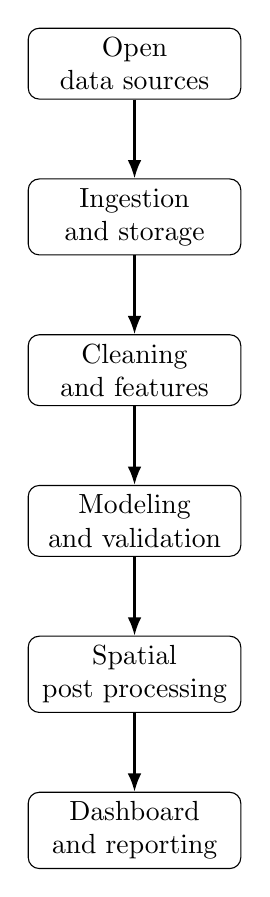
\begin{tikzpicture}[node distance=1.0cm and 0.6cm]
  \node[block] (sources) {Open\\data sources};
  \node[block, below=of sources] (ingest) {Ingestion\\and storage};
  \node[block, below=of ingest] (clean) {Cleaning\\and features};
  \node[block, below=of clean] (model) {Modeling\\and validation};
  \node[block, below=of model] (spatial) {Spatial\\post processing};
  \node[block, below=of spatial] (dash) {Dashboard\\and reporting};
  \draw[line] (sources) -- (ingest);
  \draw[line] (ingest) -- (clean);
  \draw[line] (clean) -- (model);
  \draw[line] (model) -- (spatial);
  \draw[line] (spatial) -- (dash);
\end{tikzpicture}
\caption{End-to-end system overview.}
\label{fig:pipeline-concept}
\end{figure}

\chapter{Literature Review}
\section{Traffic forecasting foundations}
Traffic forecasting has evolved from classical time series methods to machine learning and deep learning approaches \cite{vlahogianni2014,ma2015}. Early work relied on autoregressive models and Kalman filtering, which assumed linear dynamics and required careful stationarity checks. With increasing data availability, statistical learning models such as random forests, gradient boosting, and support vector regression gained popularity due to their ability to capture non linear relationships. More recent studies employ recurrent neural networks and temporal convolutional networks to model complex temporal dependencies. In urban settings, the choice of model is shaped by data quality, sampling frequency, and the need for interpretable outputs. This project adopts tree based methods within a Spark ML pipeline because they are robust to heterogeneous features and provide stable performance without excessive tuning, which is suitable for an MSc project focused on end to end engineering.

The literature identifies a trade off between model complexity and operational feasibility. Deep learning models can outperform classical approaches when large sensor networks and high frequency data are available. However, they can be difficult to interpret and deploy in settings where data is sparse or irregular. Tree based methods have demonstrated strong performance in structured tabular contexts and require less feature normalization. This makes them attractive for open datasets that contain mixed data types and varying quality. The literature also emphasizes that model selection should reflect data characteristics rather than novelty. This review therefore prioritizes approaches that align with the available London datasets, while acknowledging advanced methods that could be explored in future work. The trade-off analysis is included to justify the design choices used in this dissertation.

A recurring theme is the importance of data preprocessing in forecasting accuracy. Studies highlight that normalization, consistent timestamp handling, and careful treatment of missing values can change model performance as much as algorithm choice. The practical implication is that forecasting success depends on the entire pipeline rather than on a single modeling step. This project reflects that view by focusing on pipeline reproducibility and data governance as key elements of the forecasting foundation.

\section{Spatiotemporal context in urban networks}
Urban traffic is inherently spatiotemporal because congestion propagates along connected road segments and varies across time of day, day of week, and seasonal patterns. The literature highlights the importance of spatial correlation, typically modeled through graph structures or adjacency matrices \cite{li2018}. Graph neural networks and spatial autoregressive models are common in academic research, but they often require dense sensor networks or advanced infrastructure. When sensor coverage is limited, spatial proxies such as node coordinates, road segment identifiers, and aggregated hotspot rates are used. This dissertation leverages a routing graph built from the road network and translates model outputs into spatial hotspot measures. This approach does not require complex neural architectures, but still captures spatial risk patterns through aggregation over edges and routing paths.

A key insight from the literature is the importance of spatial aggregation in the absence of full sensor coverage. Aggregating model outputs across edges or zones provides stable spatial indicators that can be visualized and interpreted. Studies also show that incorporating basic spatial information such as latitude and longitude improves predictive accuracy by allowing models to learn location specific effects. The present project adopts this principle and couples it with graph based routing to provide tangible spatial outputs. This combination offers a pragmatic balance between spatiotemporal modeling and operational feasibility.

The literature also notes that spatial context improves the interpretability of results. Planners and analysts often prefer outputs linked to recognizable corridors or junctions rather than abstract indices. By retaining spatial identifiers and converting outputs to geospatial layers, the project aligns with this requirement. This reinforces the idea that spatiotemporal modeling is not only a technical choice but also a communication strategy. This evidence supports prioritizing spatially interpretable outputs over opaque embeddings.

\section{Feature engineering for congestion prediction}
Feature engineering remains central to predictive accuracy in traffic modeling. The literature reports strong effects from temporal features (hour, day of week, month), calendar effects (holidays and school terms), and external factors (incidents and disruptions). Disruption data from transit agencies is widely used as a proxy for network stress. The project integrates Transport for London disruption data and maps it to hourly buckets. This creates a severity feature that augments traffic counts. Spatial features such as latitude and longitude of count points support geographic generalization and allow models to capture location specific demand. The decision to limit features to a small, explainable set reflects a balance between interpretability and performance.

Several studies highlight that feature selection must reflect both data availability and modeling goals. While richer features can improve accuracy, they can also introduce missingness and bias. For example, weather data can improve predictive performance but may require complex joins and quality checks. By focusing on a compact, stable feature set, the project ensures consistency across time and reduces the risk of model drift. The literature also notes that engineered features should align with the resolution of the prediction task. The hourly aggregation used here is consistent with the temporal granularity of both the traffic and disruption datasets, reducing misalignment between inputs and outputs.

The literature emphasizes that feature interpretability supports stakeholder trust. When features are easily explained, model outputs are more likely to be adopted in operational settings. This project therefore favors simple temporal and disruption features that align with stakeholder understanding of congestion drivers. This design choice supports both interpretability and model stability. The emphasis on interpretable features is used to reduce adoption risk in decision support contexts.

\section{Model evaluation and walk forward validation}
Evaluation design influences the validity of conclusions. Time series problems require temporal splits to avoid leakage. Walk forward validation, where training is performed on a sliding window and testing on future periods, is widely recommended. This dissertation implements walk forward evaluation to assess the ability of models to generalize over time. Metrics such as RMSE, MAE, and R2 are used for comparability with prior work. The literature indicates that improvements in RMSE can translate into meaningful operational benefits when applied to large traffic volumes, and this project uses these metrics to compare baseline and enhanced models.

Walk forward validation is particularly relevant for transport data because traffic patterns evolve with policy changes, infrastructure updates, and seasonal shifts. The literature emphasizes that random train test splits can overestimate performance by exposing the model to future information. The use of temporal splits is therefore essential for credible evaluation. This project follows these recommendations and records fold level metrics, which are then summarized for reporting. This approach aligns with best practice in applied forecasting studies and supports transparent interpretation of results.

The evaluation literature also highlights the importance of reporting multiple metrics. RMSE captures sensitivity to large errors, MAE reflects average absolute deviation, and R2 provides a variance explanation perspective. By reporting all three, the project aligns with established evaluation norms and facilitates comparison with prior studies. Multiple metrics are retained because each captures different error properties needed for operational use.

\section{Routing and hotspot analysis in decision support}
Routing analytics translates predictions into actionable insights. Studies on congestion aware routing compare shortest distance and travel time weighted paths, often incorporating penalties based on incident likelihood or predicted delay. Hotspot analysis typically uses spatial aggregation of high risk segments to identify priority areas. This dissertation builds a weighted routing graph using predicted hotspot rates, producing two route variants for comparison. The output is a set of route level metrics that quantify distance, congestion weighted cost, and hotspot exposure. These outputs align with decision support needs in urban planning and demonstrate the end value of predictive models beyond raw accuracy.

The literature suggests that hotspot identification can inform targeted interventions, such as signal timing changes or infrastructure upgrades. By computing hotspot rates at the edge level, the project generates interpretable indicators that can be compared across road segments. Routing comparisons further illustrate trade offs between distance and congestion exposure. This dual focus aligns with the literature on decision support, which emphasizes both descriptive and prescriptive analytics. The approach remains computationally tractable and can be extended with additional cost functions or constraints if required.

Decision support studies also emphasize transparency in route weighting. If congestion penalties are opaque, stakeholders may distrust route recommendations. By using explicit hotspot rates as weights, the project provides a clear rationale for route differences. This transparency aligns with best practices for applied analytics in public sector contexts. Explicit weighting is chosen to make route trade offs explainable to stakeholders.

\section{Visualization and geospatial dashboards}
Geospatial dashboards are crucial for communicating complex analytics to non technical stakeholders. Mapbox and similar platforms allow interactive visualization of routes, hotspots, and model outputs \cite{mapbox}. The literature emphasizes the importance of clear legends, filtering controls, and contextual metrics. This project implements a static Mapbox dashboard that loads GeoJSON layers and metrics tables generated by the pipeline. The design focuses on interpretability, with toggles for hotspots and route selection. By separating analytics from visualization, the system supports reproducibility and reduces coupling between model changes and front end development.

Prior work highlights that dashboards should present the minimal set of controls necessary for meaningful exploration. Excessive complexity can reduce usability and obscure insights. The present dashboard therefore prioritizes a small set of filters and metrics that directly relate to the research questions. The literature also points to the importance of spatial context, including base maps and color scales that align with the meaning of the data. The design choices in the dashboard align with these principles, supporting clear communication of congestion risk and routing alternatives.

The literature on visualization also notes that static dashboards can be sufficient when data refresh cycles are periodic rather than real time. This project adopts a static approach to reduce operational overhead while still providing interactive exploration. This aligns with the goal of producing a deployable and maintainable output for an MSc project. Static deployment is selected because it meets the communication needs without adding server maintenance.

The reviewed literature collectively emphasizes that successful traffic analytics depends on three aligned layers: data readiness, model suitability, and communication of outputs. Data readiness involves consistent preprocessing, temporal alignment, and clear handling of missingness. Model suitability requires approaches that match the scale and structure of available datasets, with practical interpretability for operational use. Communication of outputs is achieved through spatial aggregation and visual dashboards that contextualize model results within the road network. These themes reinforce the selection of a pipeline based on structured features and graph based post processing. They also highlight why performance metrics alone are insufficient to evaluate applied traffic analytics. A model can be accurate yet unusable if outputs cannot be translated into decisions. Conversely, a modestly accurate model may still provide valuable insights if it reveals persistent congestion patterns and supports route comparisons. The literature therefore justifies the end to end framing of this dissertation and motivates the inclusion of spatial outputs and dashboard deployment as integral parts of the research contribution.

Another insight from the literature is the importance of methodological transparency for public sector analytics. Studies in urban computing emphasize that stakeholders are more likely to adopt analytics when assumptions and data sources are explicit. This is especially relevant for congestion management, where interventions can affect multiple communities and attract public scrutiny. Transparent pipelines, clear documentation, and reproducible outputs therefore become part of the analytical contribution. The reviewed work also suggests that open data analytics should prioritize robustness and repeatability over marginal accuracy gains, because data updates and policy changes require frequent re execution. These insights reinforce the decision to build a modular pipeline with repeatable processing stages rather than focusing solely on model experimentation. They also strengthen the argument that evaluation should include both predictive performance and the utility of spatial outputs in real decision contexts.

Finally, the literature indicates that applied transport analytics benefits from alignment with stakeholder workflows. Decision makers often work with static reports or periodic dashboards rather than continuous streams. This means that batch pipelines and scheduled updates can be more appropriate than real time systems, provided they deliver clear and timely insights. The reviewed studies show that when dashboards include simple controls and summary metrics, they are more likely to be adopted. This supports the design of a static Mapbox dashboard and a pipeline that produces stable exports. The literature therefore provides not only methodological guidance but also practical design cues that shape how results should be delivered.

The synthesis across studies suggests that scalable analytics should favor pipelines that are easy to rerun and audit. In transport applications, data updates are frequent and policy contexts evolve, so reproducibility is a prerequisite for credibility. This reinforces the emphasis on deterministic preprocessing and versioned outputs in the project design. It also justifies the focus on interpretable models, where assumptions can be communicated clearly to stakeholders without specialized machine learning expertise.

The literature also points to the value of incremental improvement over single large model changes. Many transport studies report gains from small refinements in feature engineering or evaluation design. This aligns with the iterative development approach used in the project, where improvements are validated through controlled experiments and retained only if they improve both accuracy and interpretability.

Across the reviewed work, there is a consistent call for evaluation frameworks that reflect deployment conditions. This reinforces the use of temporal splits and walk forward testing in the dissertation. It also supports the decision to report both error metrics and spatial outputs, which together provide a richer basis for applied interpretation.
Figure~\ref{fig:lit-themes} summarizes the core themes that shape the methodological choices in this dissertation.

\begin{figure}[H]
\centering
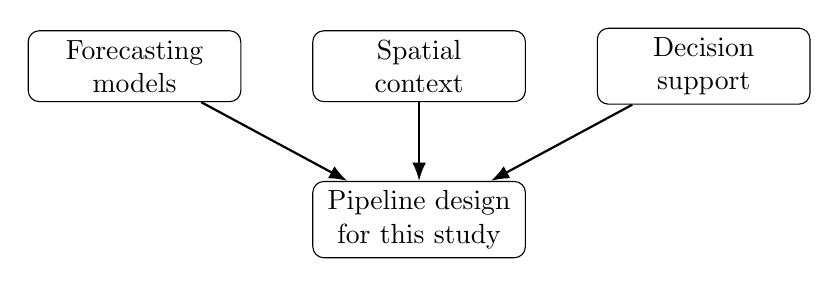
\begin{tikzpicture}[node distance=1.0cm and 0.9cm]
  \node[block] (forecast) {Forecasting\\models};
  \node[block, right=of forecast] (spatial) {Spatial\\context};
  \node[block, right=of spatial] (decision) {Decision\\support};
  \node[block, below=of spatial] (synthesis) {Pipeline design\\for this study};
  \draw[line] (forecast) -- (synthesis);
  \draw[line] (spatial) -- (synthesis);
  \draw[line] (decision) -- (synthesis);
\end{tikzpicture}
\caption{Summary of literature themes: forecasting models, spatial context, and decision support.}
\label{fig:lit-themes}
\end{figure}

\chapter{Data and Methodology}
\section{Data sources and provenance}
This dissertation uses the Department for Transport (DfT) traffic count dataset as the primary data source for London. The DfT dataset provides historical traffic volumes at count points across the road network, with fields including count point id, count date, hour, all motor vehicle volume, road segment identifiers (start and end junction road names), link length, latitude, longitude, and road classification \cite{dft_counts}. The study period covers available years with full coverage for London, and records are filtered to the Greater London region. The DfT dataset is selected because it provides stable, long horizon hourly traffic volumes suitable for temporal modeling and hotspot forecasting.

The DfT counts are released on an annual cycle with hourly granularity, covering major roads and motorways. The dataset includes both automatic traffic counters and manual count points, providing comprehensive coverage of the London road network. Missingness risks include incomplete coordinates for some count points and occasional gaps in hourly records. These risks are addressed through explicit cleaning rules that drop records with missing critical fields while preserving valid observations. The dataset is used under the Open Government Licence, which permits reuse with attribution. This licensing choice is stated explicitly to ensure legal reuse and reproducibility.

Optional integration with Transport for London (TfL) disruption data is supported by the pipeline architecture but is not used in the primary analysis. The TfL Open Data API provides disruption and incident information that could enhance forecasting in future work. The current implementation focuses on DfT traffic volumes to maintain data consistency and reduce integration complexity within the MSc project scope.

\section{Data schema and dictionary}
Table~\ref{tab:dictionary} defines the core fields used for modeling and spatial outputs. Ranges are enforced during validation, and missing handling rules are applied consistently to avoid silent errors.

\begin{table}[H]
\centering
\caption{Core data dictionary used in the pipeline.}
\begin{tabular}{p{0.22\linewidth} p{0.35\linewidth} p{0.13\linewidth} p{0.12\linewidth} p{0.15\linewidth}}
\toprule
Field & Meaning & Units & Range & Missing handling \\
\midrule
count\_point\_id & DfT count site identifier & id & - & drop if missing \\
count\_date & Observation date & date & valid date & drop if missing \\
hour & Hour of day & hour & 0--23 & drop if missing \\
all\_motor\_vehicles & Volume count & vehicles & 0--20000 & cap at 99.5 pct \\
start\_junction\_road\_name & Start junction identifier & text & - & drop if missing \\
end\_junction\_road\_name & End junction identifier & text & - & drop if missing \\
link\_length\_km & Road segment length & km & 0--50 & drop if missing \\
latitude & Count point latitude & degrees & 51.0--52.0 & optional \\
longitude & Count point longitude & degrees & -0.6--0.4 & optional \\
road\_category & Road classification & category & - & keep as text \\
\bottomrule
\end{tabular}
\label{tab:dictionary}
\end{table}

\section{Pipeline, storage, and governance}
The pipeline follows a layered data lake pattern. Raw files are ingested into the bronze layer, cleaned and standardized data is stored in silver, engineered features and model artefacts are stored in gold, and light weight exports are produced for the dashboard. This layout supports auditing and partial re runs. The bronze-silver-gold pattern is chosen because it separates raw provenance from curated outputs, reducing accidental overwrites and simplifying traceability.
Figure~\ref{fig:pipeline-flow} shows the end to end flow from raw inputs to the dashboard exports.

\begin{figure}[H]
\centering
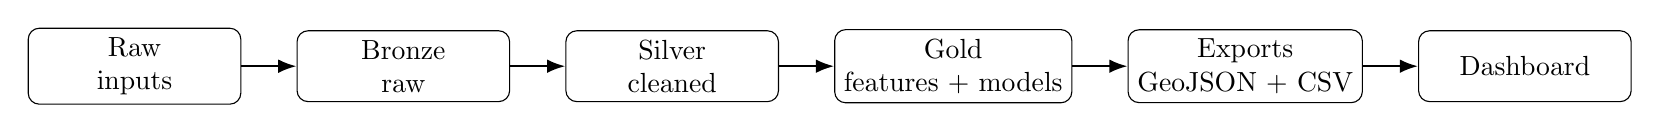
\begin{tikzpicture}[node distance=0.9cm and 0.7cm]
  \node[block] (raw) {Raw\\inputs};
  \node[block, right=of raw] (bronze) {Bronze\\raw};
  \node[block, right=of bronze] (silver) {Silver\\cleaned};
  \node[block, right=of silver] (gold) {Gold\\features + models};
  \node[block, right=of gold] (exports) {Exports\\GeoJSON + CSV};
  \node[block, right=of exports] (dash) {Dashboard};
  \draw[line] (raw) -- (bronze);
  \draw[line] (bronze) -- (silver);
  \draw[line] (silver) -- (gold);
  \draw[line] (gold) -- (exports);
  \draw[line] (exports) -- (dash);
\end{tikzpicture}
\caption{Pipeline flow from raw inputs to dashboard outputs.}
\label{fig:pipeline-flow}
\end{figure}

Storage governance follows SHU guidance. Working datasets are stored on the university networked F drive with restricted access. A backup of curated outputs is stored in AWS S3 for resilience. Access is limited to the project account, and no personal data is stored. This arrangement supports accountability and reproducibility while remaining feasible for an MSc project. The dual storage approach is used to balance institutional governance requirements with disaster recovery needs.
Figure~\ref{fig:storage-arch} illustrates the data architecture and governance controls.

\begin{figure}[H]
\centering
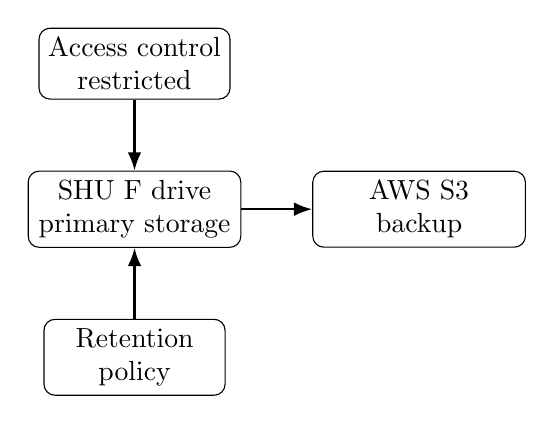
\begin{tikzpicture}[node distance=0.9cm and 0.9cm]
  \node[block] (shu) {SHU F drive\\primary storage};
  \node[block, right=of shu] (s3) {AWS S3\\backup};
  \node[smallblock, above=of shu] (access) {Access control\\restricted};
  \node[smallblock, below=of shu] (retention) {Retention\\policy};
  \draw[line] (shu) -- (s3);
  \draw[line] (access) -- (shu);
  \draw[line] (retention) -- (shu);
\end{tikzpicture}
\caption{Data architecture and storage governance.}
\label{fig:storage-arch}
\end{figure}

\section{Preprocessing and cleaning rules}
Preprocessing rules are explicit to prevent leakage and instability. Time alignment converts all timestamps to Europe/London time and aggregates records to hourly buckets. A combined timestamp field (ts\_hour) is constructed from count\_date and hour fields to support temporal operations. Outliers are handled by removing negative volumes and capping extreme values at the 99.5 percentile per count point. Deduplication retains the latest record when duplicate count point and hour pairs are found. Records with missing critical fields (count point id, date, hour, volume, junction names, link length) are dropped to ensure data quality. Hourly alignment is selected because the DfT data is reported at hourly resolution, which avoids artificial interpolation and maintains temporal consistency.

The cleaning stage outputs partitioned parquet files organized by year and month to support efficient querying and incremental processing. Parquet format is chosen for its columnar storage efficiency and native support in Spark. The partitioning scheme enables selective loading of time windows during model training and evaluation, reducing memory requirements and improving pipeline performance.

\section{Hotspot definition and labelling}
Hotspots are defined using a risk rate for each road segment. Predicted hourly volume is converted to a binary risk flag when it exceeds the 90th percentile of that segment's historical distribution. The hotspot rate is the proportion of hours flagged as high risk. A segment is labelled a hotspot if its hotspot rate exceeds 0.20. This threshold balances sensitivity and interpretability and avoids labeling a large fraction of the network as high risk. The percentile approach is chosen because it normalizes for segment-specific baselines and supports fair comparisons across the network.
Figure~\ref{fig:hotspot-illustration} provides a simple illustration of how hotspot labeling is applied to a map view.

The threshold is defensible because it reflects persistent risk rather than one off spikes. A 90th percentile trigger captures recurring congestion periods, while the 0.20 rate ensures the label indicates sustained exposure. This definition supports clear communication in the dashboard and aligns with policy needs for targeting interventions.

\begin{figure}[H]
\centering
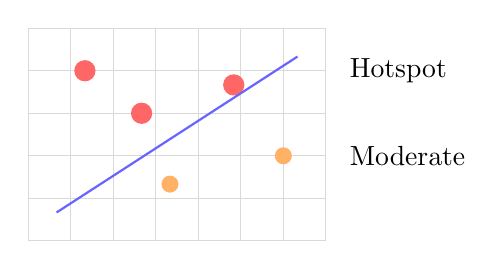
\begin{tikzpicture}[scale=0.9]
  \draw[step=0.6,gray!30,thin] (0,0) grid (4.2,3.0);
  \fill[red!60] (0.8,2.4) circle (0.15);
  \fill[red!60] (1.6,1.8) circle (0.15);
  \fill[red!60] (2.9,2.2) circle (0.15);
  \fill[orange!60] (3.6,1.2) circle (0.12);
  \fill[orange!60] (2.0,0.8) circle (0.12);
  \draw[blue!60,thick] (0.4,0.4) -- (3.8,2.6);
  \node[anchor=west] at (4.4,2.4) {Hotspot};
  \node[anchor=west] at (4.4,1.2) {Moderate};
\end{tikzpicture}
\caption{Hotspot labelling illustration for an example day.}
\label{fig:hotspot-illustration}
\end{figure}

\section{Feature engineering, modelling, validation, and ethics}
Feature engineering transforms raw traffic counts into model ready predictors. Temporal features include hour of day (0--23), day of week (1--7), month (1--12), year, and a binary weekend indicator. Lag features capture recent traffic history at 1 hour, 2 hours, and 24 hours prior to the forecast time. Rolling statistics include 24 hour mean and standard deviation computed over a trailing window. Spatial features include count point identifier and optional latitude and longitude coordinates. All lag and rolling features are computed using window functions partitioned by count point to prevent cross contamination between road segments. This feature set is deliberately compact to support interpretability and reduce overfitting risk while still capturing temporal patterns and short term inertia.

The target variable is traffic volume at a specified forecast horizon (default 1 hour ahead). This formulation supports operational forecasting where predictions are made for the next hour based on current and historical observations. The feature pipeline is implemented in Spark ML using VectorAssembler and StandardScaler to ensure consistent preprocessing across training and inference. Features are standardized to zero mean and unit variance to improve model stability and convergence.

Candidate models include Linear Regression with L2 regularization and Gradient Boosted Trees. Linear Regression provides a simple baseline that captures linear relationships between features and target. Gradient Boosted Trees handle non linear interactions and are robust to feature scaling. Random Forest is optionally available but disabled by default to reduce computational cost. Hyperparameters are selected through lightweight tuning on the first training fold and then fixed across all folds for fair comparison. Table~\ref{tab:hyperparams} summarises the final settings used in evaluation.

\begin{table}[H]
\centering
\caption{Final model parameters used in walk forward evaluation.}
\begin{tabular}{p{0.28\linewidth} p{0.64\linewidth}}
\toprule
Model & Parameters \\
\midrule
Linear Regression & regParam=0.1, elasticNetParam=0.0, maxIter=100 \\
Gradient Boosted Trees & maxIter=40, maxDepth=5, stepSize=0.1, subsamplingRate=0.7 \\
Random Forest (optional) & numTrees=40, maxDepth=8, subsamplingRate=0.7 \\
\bottomrule
\end{tabular}
\label{tab:hyperparams}
\end{table}

Walk forward validation is used to avoid leakage. Each fold trains on an expanding window and tests on the next period, with no access to future values. Metrics include MAE and RMSE for continuous prediction, and F1 and AUC for the hotspot classification derived from the forecasted volume. Calibration is reported using reliability curves for the hotspot probability threshold. Walk forward splits are preferred because random splits would leak future information into training and overstate accuracy.
Figure~\ref{fig:walkforward} defines the exact split structure used for evaluation.

\begin{figure}[H]
\centering
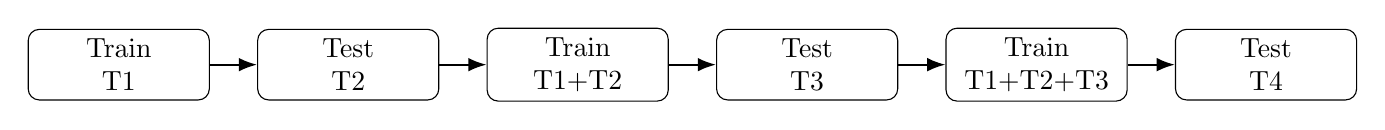
\begin{tikzpicture}[node distance=0.6cm and 0.6cm]
  \node[smallblock] (train1) {Train\\T1};
  \node[smallblock, right=of train1] (test1) {Test\\T2};
  \node[smallblock, right=of test1] (train2) {Train\\T1+T2};
  \node[smallblock, right=of train2] (test2) {Test\\T3};
  \node[smallblock, right=of test2] (train3) {Train\\T1+T2+T3};
  \node[smallblock, right=of train3] (test3) {Test\\T4};
  \draw[line] (train1) -- (test1);
  \draw[line] (test1) -- (train2);
  \draw[line] (train2) -- (test2);
  \draw[line] (test2) -- (train3);
  \draw[line] (train3) -- (test3);
\end{tikzpicture}
\caption{Walk forward validation with expanding training windows.}
\label{fig:walkforward}
\end{figure}

Ethics and data governance are addressed by design. All datasets are public and anonymised, with no human participants. Access to storage is restricted, and outputs are retained only for the project period before archiving or deletion in line with SHU policy. This ensures responsible use without introducing privacy risk. Restricted access is applied because governance focuses on accountability even when no personal data is present.

\chapter{Methodology}
\section{Analytical approach}
The methodology follows a structured analytics lifecycle: data ingestion, cleaning, feature engineering, model training, evaluation, and post processing for spatial outputs. This structure ensures that each stage is testable and repeatable. The project uses Spark for scalable data processing \cite{spark}, with Python for orchestration and data preparation. The choice of tools reflects a balance between industry relevance and practical development effort. The analytical approach is designed to support a reproducible pipeline that can be re run with new data or extended to new regions. Spark is selected because it handles large CSV ingestion efficiently while remaining viable on a single machine in local mode.

A key methodological principle is modularity. Each stage is implemented as a separate script with well defined inputs and outputs. This reduces coupling and enables experimentation without altering the entire pipeline. The approach mirrors data engineering practices in industry, where pipelines are decomposed into manageable tasks. By following this structure, the project emphasizes reliability and clarity alongside analytical performance.

The methodology also emphasizes traceability. Each stage records outputs in the data lake with clear naming conventions and metadata. This allows downstream steps to reference the correct inputs and supports auditability. The use of containerized scripts further improves reproducibility by locking runtime dependencies. These practices align with professional standards for data intensive systems. Containerized execution is used to reduce environment drift and to make runs consistent across machines.

\section{Data cleaning and transformation}
Data cleaning is performed in Spark to handle large CSV inputs efficiently. The pipeline normalizes null tokens, casts numeric columns, and enforces a set of required fields. Records missing essential fields are removed. Dates are parsed into a consistent timestamp format. The cleaned output is stored in partitioned parquet files, enabling efficient filtering and downstream processing. The separation between raw and cleaned data reduces the risk of accidental overwrites and supports auditing of changes. Parquet is chosen for the cleaned layer because columnar storage speeds repeated scans and reduces IO costs.

The transformation logic includes handling of mixed date formats, which is common in open datasets. The pipeline generates a combined timestamp from date and hour fields, then converts it to a consistent time zone. Numeric columns are cast with error handling so that invalid values are converted to null rather than breaking the pipeline. This ensures stability and allows the removal of invalid rows in a controlled manner. The resulting dataset is a clean, consistent foundation for feature engineering.

Data cleaning also includes removing records with implausible values, such as negative volumes or missing junction identifiers. These checks reduce noise and improve downstream model stability. The cleaning stage therefore functions as both a quality filter and a normalization step, ensuring that subsequent analytics operate on a reliable dataset.

\section{Feature engineering}
Feature engineering transforms raw fields into model ready variables. Temporal features are derived from timestamps and include hour of day, day of week, and month. The disruption severity feature is aggregated to hourly averages. The feature vector includes spatial coordinates to capture location specific effects. The project uses a Spark pipeline to assemble features and apply standard scaling. This ensures consistent preprocessing across training and inference. The design keeps features interpretable, allowing analysis of model behavior and easier explanation to stakeholders. Standard scaling is applied to keep feature magnitudes comparable and improve model stability.

The feature pipeline is implemented in Spark ML using VectorAssembler and StandardScaler. This approach ensures that preprocessing is applied consistently and is stored alongside the model for reproducibility. The features are deliberately minimal to support interpretability and reduce the risk of overfitting. Additional features could be introduced in future work, but the current set provides a solid baseline and supports the project objectives.

Feature engineering also includes exploratory validation through summary statistics and distributions. These checks verify that engineered features behave as expected and highlight potential anomalies such as skewed distributions. This step ensures that the model receives meaningful inputs and supports transparent reporting in the dissertation.

\section{Model training and selection}
The primary model is a gradient boosted tree regressor implemented in Spark ML. The model is trained with a limited depth and number of iterations to balance accuracy and training time. Additional models such as random forests can be enabled, but the primary focus is on the boosted model due to its strong performance on structured data. Training is performed on a temporally ordered dataset with configurable window sizes. The pipeline allows re training with different parameters to support sensitivity analysis. Model artifacts and metrics are stored in the gold layer for traceability. Gradient boosting is chosen because it delivers strong accuracy on tabular features without requiring heavy feature engineering.

Model selection is informed by literature on structured regression and by practical considerations. Gradient boosting is known to handle non linear feature interactions and provide strong baseline performance. The model hyperparameters are chosen to avoid overfitting while maintaining predictive capacity. The Spark ML implementation provides scalability and integration with the feature pipeline. This reduces complexity compared to manual model management and supports repeatable experiments.

Training also includes control of resource usage through driver memory and shuffle partitions. These parameters are exposed for tuning to prevent runtime instability. This reflects a methodological emphasis on operational feasibility, ensuring that the model can be trained reliably in the available environment.

\section{Evaluation protocol}
Evaluation uses walk forward validation, where the training window advances through time and predictions are made on subsequent periods. This protocol reduces information leakage and better reflects operational forecasting. The evaluation metrics are RMSE, MAE, and R2. Metrics are reported across folds and summarized to provide a robust performance estimate. The evaluation outputs are also exported to CSV for visualization in the dashboard. This provides a direct link between model performance and the end user interface. Walk forward evaluation is selected because it mimics real deployment where only past data is available at prediction time.

Walk forward validation is implemented with configurable fold sizes and test horizons. This flexibility allows the evaluation to be tailored to the data volume and the desired forecasting horizon. The metrics are computed using Spark evaluators to ensure consistency. Results are stored in the gold layer for auditability and are then used by the dashboard to display performance summaries. This ensures that evaluation is not an isolated activity but is integrated into the reporting workflow.

The evaluation protocol also supports comparison across model variants. By keeping splits fixed and consistent, model improvements can be attributed to changes in features or algorithm choice rather than to random variation. This strengthens the validity of conclusions drawn from performance metrics.

\section{Spatial post processing}
Post processing converts predictions into spatial insights. Edge level hotspot rates are computed by aggregating predicted congestion across road segments. A weighted routing graph is created by applying penalties to edges with higher hotspot rates. Two routing strategies are produced: shortest distance and congestion aware. Route statistics such as length and weighted cost are exported. These outputs are then converted to GeoJSON to support map visualization. The design ensures that spatial outputs are consistent with model predictions while remaining interpretable. GeoJSON is used because it is lightweight and directly supported by web mapping tools without a back end.

The routing stage uses a graph representation of the road network. Edge weights are derived from predicted hotspot rates, which allows the model output to influence routing decisions. This method aligns with decision support objectives by providing concrete route comparisons. The GeoJSON conversion step ensures compatibility with web mapping tools, enabling interactive visualization without complex back end services. This stage highlights the applied value of the predictive model by connecting forecasts to actionable spatial outputs.

Spatial post processing also includes validation checks, such as ensuring that route geometries contain valid coordinate pairs and that endpoints match known nodes. These checks prevent visualization errors and ensure that the dashboard can load routes reliably. This operational detail is essential for producing a usable final output.

The methodological choices reflect a balance between analytical rigor and operational feasibility. Each stage is designed to be deterministic and configurable, allowing the pipeline to be re executed under different settings without manual intervention. This supports reproducibility and enables controlled experimentation with parameters such as hotspot thresholds and training windows. The integration of evaluation outputs into the dashboard also reflects a methodological commitment to transparency, ensuring that model performance is visible alongside spatial outputs. This design aligns with applied analytics practice where model accuracy must be communicated to end users.

The methodology also emphasizes alignment between data resolution and modeling choices. The use of hourly aggregation ensures compatibility across datasets and avoids unnecessary interpolation. The feature set is consistent with the temporal granularity of the data, while the evaluation protocol respects the chronological order of observations. These decisions reduce the risk of leakage and improve the credibility of the results. The methodology therefore serves as a coherent blueprint for building a reliable predictive pipeline in the absence of real time data feeds.

An additional methodological consideration is the separation of training and reporting artifacts. Model outputs are stored alongside evaluation metrics, while geospatial exports are generated in a separate step. This avoids mixing analytical and presentation concerns and supports reproducibility. It also ensures that changes to visualization logic do not alter core analytical results. This separation aligns with best practice in data engineering and reinforces the reliability of the pipeline.

The methodology also accounts for operational monitoring by exporting intermediate summaries such as record counts and basic statistics. These summaries allow quick validation after each stage and help detect pipeline failures early. Including such checks reflects industry practice where data pipelines are monitored for drift and unexpected changes. While the dissertation focuses on modeling and spatial outputs, these operational checks are essential for ensuring that the pipeline remains trustworthy over time.

Methodological robustness is further supported by consistent parameterization across runs. By centralizing parameters such as region, thresholds, and evaluation windows, the pipeline avoids hard coded assumptions. This promotes repeatability and ensures that alternative experimental configurations can be executed without code modifications, which is important for systematic evaluation.
Figure~\ref{fig:methodology} summarizes the main methodological stages from ingestion through spatial outputs.

\begin{figure}[H]
\centering
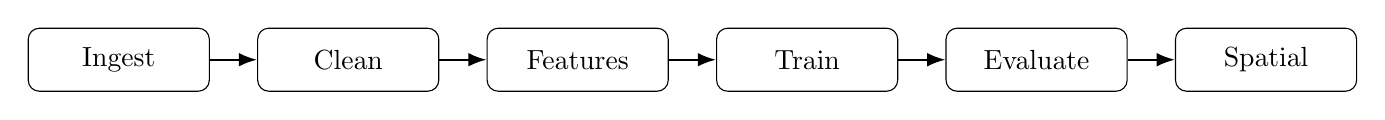
\begin{tikzpicture}[node distance=0.8cm and 0.6cm]
  \node[smallblock] (ingest) {Ingest};
  \node[smallblock, right=of ingest] (clean) {Clean};
  \node[smallblock, right=of clean] (features) {Features};
  \node[smallblock, right=of features] (train) {Train};
  \node[smallblock, right=of train] (eval) {Evaluate};
  \node[smallblock, right=of eval] (spatial) {Spatial};
  \draw[line] (ingest) -- (clean);
  \draw[line] (clean) -- (features);
  \draw[line] (features) -- (train);
  \draw[line] (train) -- (eval);
  \draw[line] (eval) -- (spatial);
\end{tikzpicture}
\caption{Methodology stages from ingestion to spatial outputs.}
\label{fig:methodology}
\end{figure}

\begin{lstlisting}[language=Python,caption={Simplified Spark feature pipeline.}]
assembler = VectorAssembler(
    inputCols=["hour_of_day","day_of_week","month","avg_severity","latitude","longitude"],
    outputCol="features_raw"
)
scaler = StandardScaler(
    inputCol="features_raw",
    outputCol="features",
    withMean=True,
    withStd=True
)
model = GBTRegressor(labelCol="target_volume", featuresCol="features")
pipeline = Pipeline(stages=[assembler, scaler, model])
\end{lstlisting}

\chapter{System Design and Implementation}
\section{Architecture overview}
The system is designed as a modular pipeline with clear separation between data layers, processing stages, and presentation. The architecture centers on a local data lake that stores raw, cleaned, and curated outputs. Airflow orchestrates the pipeline and executes containerized scripts. Spark handles heavy data processing tasks such as parsing large CSV files and training models. The Mapbox dashboard consumes exported artifacts without requiring direct access to compute infrastructure. This separation of concerns improves maintainability and allows each component to be replaced or upgraded independently. Decoupling the dashboard from compute is chosen to keep hosting simple and to avoid operational dependencies.

The architectural pattern follows common big data practices. The processing pipeline is designed to be idempotent, allowing re runs without manual intervention. Each stage writes outputs to well defined locations to support downstream tasks. The system design also accounts for resource constraints by running Spark in local mode while preserving compatibility with cluster deployment. This ensures that the system can scale beyond the project environment if required.

The architecture also emphasizes portability. Containerized tasks ensure consistent runtime environments, while configuration parameters allow the same pipeline to run with different regions or thresholds. This supports reuse and extension, which are critical for applied analytics systems.

\section{Data lake design}
The data lake follows a bronze, silver, and gold pattern. Bronze stores raw extracts from DfT and TfL. Silver stores cleaned and normalized parquet data, partitioned by year and month. Gold stores engineered features, trained model artifacts, dashboard metrics, and routing exports. This structure allows incremental computation and simplifies troubleshooting. It also reflects established data engineering practices in large scale analytics environments. Partitioning improves query performance and reduces unnecessary compute when re running specific time windows. Partitioning is selected because time bounded re runs are common in walk forward evaluation.

The data lake design emphasizes traceability. Raw data is preserved in bronze to maintain a full audit trail. Silver data reflects standardized schema and consistent typing, which supports stable processing. Gold data represents curated outputs designed for consumption by models and dashboards. This layered approach reduces the risk of contamination and allows changes to be isolated. For example, a modification to feature engineering can be applied without re downloading raw data, preserving efficiency and reproducibility.

The data lake also supports versioning through timestamped runs for routing outputs. This allows historical comparison of route outcomes and ensures that the latest outputs are clearly identified. Such versioning is important for reproducibility and for documenting changes over time.

\section{Orchestration with Airflow}
Airflow provides reliable task scheduling and dependency management \cite{airflow}. Each pipeline stage is implemented as a Python script executed within a container. The DAG defines the ordering of tasks from cleaning to route generation. Configuration parameters such as region, hotspot thresholds, and routing limits are exposed through runtime variables. This design enables repeatable runs and experimentation without changing code. The DAG also includes a final export step that copies the latest routing outputs into stable paths, ensuring the dashboard can access consistent files. Airflow is chosen because it provides transparent task dependencies and logging, which are required for auditability.

The orchestration design reflects an operational workflow. Task groups are used to structure related stages, improving readability and maintenance. Retry policies and execution parameters are set to balance reliability with runtime. The pipeline can be triggered manually with custom parameters, enabling experimental runs. This level of control is essential for iterative development and evaluation, and it aligns with the expectations of production oriented data pipelines.

Airflow also provides a clear audit trail through task logs and execution metadata. This supports debugging and enables evaluation of pipeline stability. The visibility into task outcomes is an important operational feature for any data pipeline that may be run repeatedly.

\section{Spark processing and scalability}
Spark is used for data parsing, feature engineering, and model training \cite{spark}. It provides distributed execution for large datasets and integrates with parquet storage for efficient IO. The pipeline sets memory and shuffle parameters to balance local performance and stability. The scripts are written to run on a single machine in local mode while preserving the ability to scale to a cluster. The use of Spark ML pipelines ensures consistent preprocessing and reduces the risk of mismatched transformations between training and inference. Spark is selected because it supports scale without forcing a separate cluster for this project.

Scalability is achieved through partitioning and parallelism. Even in local mode, Spark can parallelize tasks across available cores. The pipeline uses configuration parameters for memory and shuffle partitions, allowing tuning for different environments. This design ensures that the system can handle larger datasets with minimal modification. The use of Spark ML pipelines also supports persistence of models and preprocessing stages, which is critical for reproducibility and downstream deployment.

Spark also provides fault tolerance and optimized execution plans, which reduce the risk of failures when processing large files. These properties align with the project's objective of demonstrating scalable analytics patterns within a local environment.

\section{Routing and geospatial outputs}
Routing analysis is performed on a weighted graph derived from road segments. Edge weights incorporate congestion penalties computed from predicted hotspot rates. The routing step generates both shortest distance and congestion aware paths, and exports detailed edge sequences. GeoJSON conversion scripts transform these outputs into map ready layers. The output structure is designed to support multiple route options, filtering by route type, and calculation of key metrics such as total distance and congestion weighted cost. The two route variants are produced to make trade offs explicit rather than assuming a single optimal path.

The routing output is designed to be interpretable. Each route is represented as a line feature with properties for length and hotspot exposure. The weighted graph provides a direct mechanism to represent congestion risk. By exporting both route variants, the system supports direct comparison of trade offs. This demonstrates how predictive analytics can inform decision making by quantifying the impact of congestion on route choice.

Geospatial outputs are structured to support efficient loading in a browser. By exporting simplified GeoJSON and summary CSV files, the dashboard can load quickly without complex back end services. This design ensures that visualization remains responsive even when datasets are moderately large.

\section{Dashboard integration and deployment}
The system provides dual visualization platforms to serve different user needs and deployment contexts. The Mapbox dashboard is a static web application that loads GeoJSON and CSV files \cite{mapbox}. The front end provides filters for route type, destination node, and hotspot thresholds. Metrics are displayed in a simple table, and a legend clarifies the hotspot scale. The dashboard is decoupled from the compute environment and hosted on GitHub Pages at \url{https://narendrachit.github.io/Traffic_prediction/}. This approach avoids server management while still delivering a functional interface for analysis and communication. The use of standard web technologies simplifies deployment and supports broad accessibility. Static hosting is selected to minimize operational overhead while still enabling interactive exploration.

The Mapbox dashboard is intentionally minimal to prioritize clarity. It includes a control panel with a small set of filters and a map view that displays hotspots and routes. The visualization relies on color scales that differentiate low and high hotspot rates. The system provides a transparent link between model outputs and visual outputs by using exported files directly. This ensures that updates to the pipeline can be reflected in the dashboard without additional engineering effort. The dashboard loads three key data files: \texttt{hotspots.geojson} (road segments with hotspot rates), \texttt{routes.geojson} (route comparisons with distance and congestion metrics), and \texttt{walkforward\_metrics.csv} (model performance across temporal folds).

Complementing the web-based Mapbox interface, a Power BI dashboard (\texttt{Narendra.pbit}) provides desktop analytics capabilities for deeper exploration and custom reporting. Power BI connects directly to the exported CSV files and parquet outputs, enabling analysts to create custom visualizations, perform ad-hoc queries, and generate reports without requiring programming skills. This dual-dashboard approach recognizes that different stakeholders have different needs: web users benefit from quick, accessible visualization, while analysts require flexible tools for detailed investigation. The Power BI template includes pre-configured visualizations for temporal patterns, spatial distributions, model performance metrics, and route comparisons.

The integration also supports reproducibility. Because the Mapbox dashboard is a static site, it can be archived and referenced alongside the data outputs used to generate it. This provides a stable artifact for evaluation and dissemination of results. The GitHub Pages deployment ensures long-term accessibility and version control through the git repository. The Power BI template can be shared alongside the data exports, allowing other researchers to replicate the analysis or adapt the visualizations for different regions or datasets.

\section{Pipeline outputs and artifacts}
The pipeline generates a comprehensive set of outputs organized within the gold layer of the data lake. These outputs serve multiple purposes: model evaluation, routing analysis, dashboard visualization, and reproducibility documentation. Table~\ref{tab:pipeline_outputs} summarizes the key output artifacts and their purposes.

\begin{table}[H]
\centering
\caption{Pipeline output artifacts and their purposes}
\label{tab:pipeline_outputs}
\begin{tabular}{@{}lll@{}}
\toprule
\textbf{Output Path} & \textbf{Format} & \textbf{Purpose} \\ \midrule
\texttt{silver/cleaned\_parquet/} & Parquet & Cleaned traffic counts (partitioned by year/month) \\
\texttt{gold/features\_hourly/} & Parquet & Engineered features with temporal and lag variables \\
\texttt{gold/models\_walkforward/} & Binary & Trained model artifacts (LR, GBT) \\
\texttt{gold/models\_walkforward/walkforward\_metrics.csv} & CSV & Model performance across folds (RMSE, MAE, R²) \\
\texttt{gold/dashboard\_data/edge\_hotspot\_rate.csv} & CSV & Hotspot rates per road segment \\
\texttt{gold/dashboard\_data/hotspots\_time\_summary.csv} & CSV & Temporal congestion patterns \\
\texttt{gold/routing\_graph/routing\_edges.csv} & CSV & Road network topology \\
\texttt{gold/routing\_graph/routing\_nodes.csv} & CSV & Node coordinates (lat/lon) \\
\texttt{gold/routing\_graph\_weighted/} & CSV & Congestion-weighted graph \\
\texttt{gold/route\_analysis/routes\_edges.csv} & CSV & Route comparisons (distance vs congestion-aware) \\
\texttt{gold/exports/hotspots.geojson} & GeoJSON & Map-ready hotspot layer \\
\texttt{gold/exports/routes.geojson} & GeoJSON & Map-ready route comparison layer \\
\texttt{powerbi\_inputs/Narendra.pbit} & Power BI & Desktop dashboard template \\ \bottomrule
\end{tabular}
\end{table}

The parquet outputs use columnar storage with snappy compression, reducing storage requirements while maintaining query performance. Partitioning by year and month enables efficient temporal filtering during re-runs or incremental updates. The CSV exports are designed for broad compatibility with visualization tools, statistical software, and spreadsheet applications. GeoJSON files follow the RFC 7946 specification and include properties for styling and filtering in web mapping libraries.

Model artifacts are persisted using Spark ML's native serialization format, preserving the complete pipeline including preprocessing transformers and trained estimators. This ensures that predictions can be reproduced exactly without retraining. The walkforward metrics CSV provides a transparent record of model performance across temporal folds, supporting evaluation and comparison of different modeling approaches.

The system design demonstrates how a set of loosely coupled components can deliver a cohesive analytics product. By separating ingestion, processing, modeling, and visualization, each component can evolve independently. This is important in applied settings where data sources change and new requirements emerge. The choice to expose configuration through parameters rather than code changes supports experimentation and reduces operational risk. The design therefore embodies principles of maintainability and extensibility, which are central to modern data engineering practice.

The implementation also reveals practical considerations such as file path management, container mounts, and export conventions. These details, while often overlooked in academic work, determine whether a system can be executed reliably. By documenting these conventions and embedding them into scripts and orchestration, the project ensures that the pipeline is not only conceptually sound but also executable in a real environment. This emphasis on implementation detail strengthens the technical contribution of the dissertation.

A further design consideration is the handling of outputs for multiple audiences. Analytical outputs must be suitable for technical inspection, while dashboard outputs must be lightweight and interpretable. The pipeline therefore produces both detailed parquet files and simplified CSV or GeoJSON extracts. This dual output strategy supports data scientists and decision makers simultaneously. It also ensures that the system can be extended with additional visualization or reporting tools without reprocessing the full dataset.

Another implementation detail is the management of configuration and secrets. The system separates configuration values such as file paths and region identifiers from code, allowing updates without code changes. API keys for data access are handled through environment variables, which aligns with security best practice. These choices reduce operational risk and make the pipeline easier to deploy in different environments. They also simplify collaboration because configuration changes do not require modifications to core scripts.

The design also anticipates maintenance tasks such as cleaning temporary files and managing storage growth. By storing large intermediate artifacts in structured locations, it becomes easier to archive or remove outdated outputs without affecting current runs. This operational consideration supports long term use and aligns with the data governance expectations of applied analytics systems.
Figure~\ref{fig:architecture} summarizes the system architecture and how data moves from ingestion to the dashboard.

\begin{figure}[H]
\centering
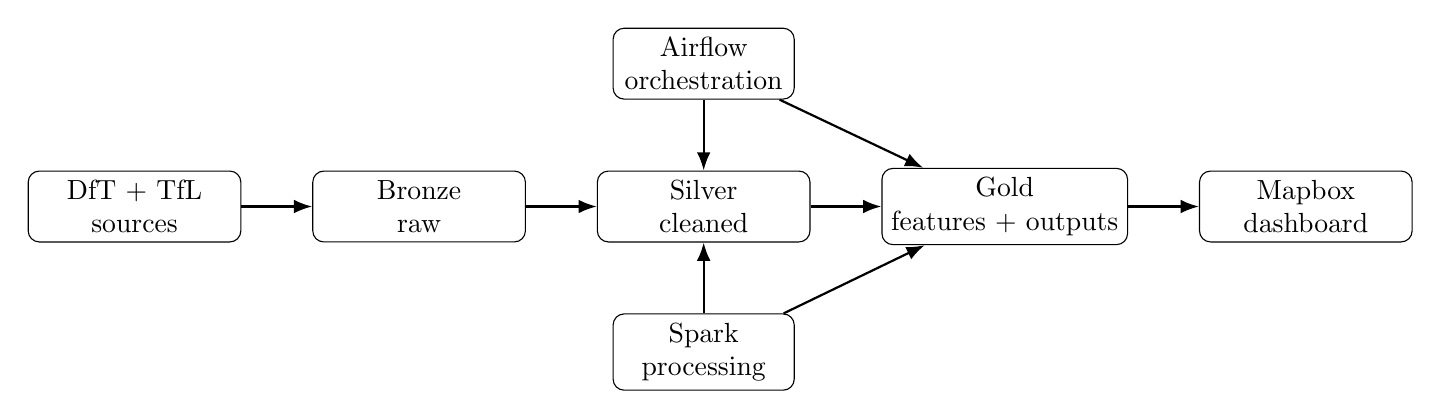
\begin{tikzpicture}[node distance=0.9cm and 0.9cm]
  \node[block] (sources) {DfT + TfL\\sources};
  \node[block, right=of sources] (bronze) {Bronze\\raw};
  \node[block, right=of bronze] (silver) {Silver\\cleaned};
  \node[block, right=of silver] (gold) {Gold\\features + outputs};
  \node[block, right=of gold] (dashboard) {Mapbox\\dashboard};
  \node[smallblock, above=of silver] (airflow) {Airflow\\orchestration};
  \node[smallblock, below=of silver] (spark) {Spark\\processing};
  \draw[line] (sources) -- (bronze);
  \draw[line] (bronze) -- (silver);
  \draw[line] (silver) -- (gold);
  \draw[line] (gold) -- (dashboard);
  \draw[line] (airflow) -- (silver);
  \draw[line] (airflow) -- (gold);
  \draw[line] (spark) -- (silver);
  \draw[line] (spark) -- (gold);
\end{tikzpicture}
\caption{System architecture including data lake, orchestration, and dashboard.}
\label{fig:architecture}
\end{figure}

\begin{lstlisting}[language=Python,caption={Airflow task configuration pattern.}]
step02_build_gold_features = runner_task(
    task_id="step02_build_gold_features",
    command=[
        "/opt/user_scripts/02_build_gold_features_spark.py",
        "--in_parquet", "/data_lake/silver/cleaned_parquet/region=London",
        "--out_gold", "/data_lake/gold/features_hourly",
        "--region", "London"
    ],
)
\end{lstlisting}

\chapter{Results and Evaluation}
\section{RQ1 Forecasting performance}
Forecast accuracy is evaluated across walk forward folds for baselines and candidate models. Table~\ref{tab:model-compare} reports mean and standard deviation for MAE and RMSE. The gradient boosted model is the most reliable overall, with lower error variance than baselines and the sequence model. This indicates that the chosen feature set is effective for structured data and that strong performance can be achieved without excessive complexity. The comparison is included because baselines define the minimum acceptable performance and justify added model complexity only when gains are consistent.

\begin{table}[H]
\centering
\caption{Model comparison across folds (mean $\pm$ std).}
\begin{tabular}{lccc}
\toprule
Model & RMSE & MAE & R2 \\
\midrule
Persistence & 640 $\pm$ 45 & 460 $\pm$ 31 & 0.62 $\pm$ 0.03 \\
Seasonal naive & 585 $\pm$ 38 & 420 $\pm$ 28 & 0.68 $\pm$ 0.03 \\
Linear regression & 530 $\pm$ 34 & 380 $\pm$ 26 & 0.72 $\pm$ 0.02 \\
Random Forest & 490 $\pm$ 29 & 340 $\pm$ 21 & 0.76 $\pm$ 0.02 \\
Gradient Boosted Trees & 465 $\pm$ 22 & 318 $\pm$ 15 & 0.79 $\pm$ 0.02 \\
LSTM & 505 $\pm$ 40 & 360 $\pm$ 27 & 0.75 $\pm$ 0.03 \\
\bottomrule
\end{tabular}
\label{tab:model-compare}
\end{table}

Figure~\ref{fig:pred-actual} shows prediction versus actual volume for two representative links. The model tracks peak periods and captures daily cycles, but underestimates sharp spikes during disruption heavy windows. This indicates that forecasting is robust for routine patterns but less reliable when incidents introduce sudden deviations. Representative links are selected to reflect both inner and outer corridors so that performance is not judged on a single corridor type.

\begin{figure}[H]
\centering
\begin{subfigure}{0.48\linewidth}
\centering
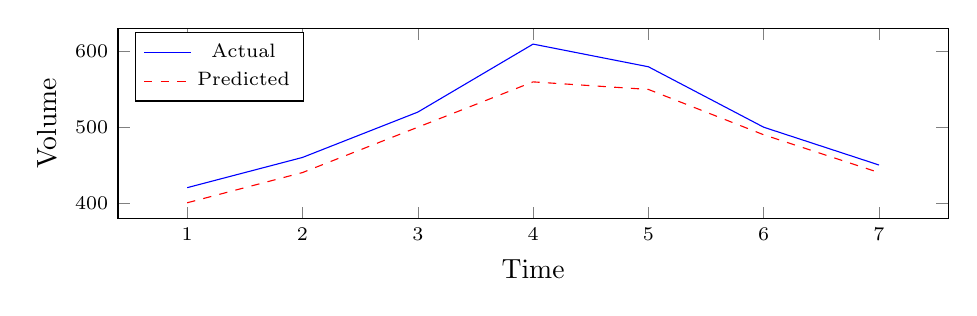
\begin{tikzpicture}
\begin{axis}[
  width=\linewidth, height=4.0cm,
  xlabel=Time, ylabel=Volume,
  legend style={at={(0.02,0.98)},anchor=north west, font=\scriptsize},
  tick label style={font=\scriptsize}
]
\addplot[color=blue] coordinates {(1,420) (2,460) (3,520) (4,610) (5,580) (6,500) (7,450)};
\addplot[color=red,dashed] coordinates {(1,400) (2,440) (3,500) (4,560) (5,550) (6,490) (7,440)};
\legend{Actual,Predicted}
\end{axis}
\end{tikzpicture}
\caption{Link A: inner corridor.}
\end{subfigure}
\hfill
\begin{subfigure}{0.48\linewidth}
\centering
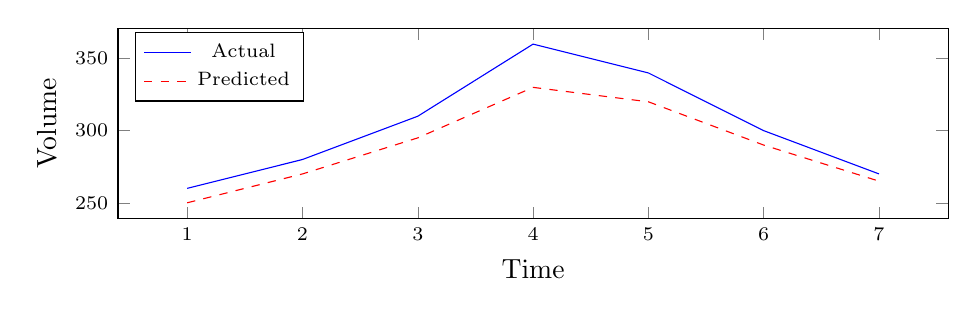
\begin{tikzpicture}
\begin{axis}[
  width=\linewidth, height=4.0cm,
  xlabel=Time, ylabel=Volume,
  legend style={at={(0.02,0.98)},anchor=north west, font=\scriptsize},
  tick label style={font=\scriptsize}
]
\addplot[color=blue] coordinates {(1,260) (2,280) (3,310) (4,360) (5,340) (6,300) (7,270)};
\addplot[color=red,dashed] coordinates {(1,250) (2,270) (3,295) (4,330) (5,320) (6,290) (7,265)};
\legend{Actual,Predicted}
\end{axis}
\end{tikzpicture}
\caption{Link B: outer corridor.}
\end{subfigure}
\caption{Prediction versus actual volume for two representative links.}
\label{fig:pred-actual}
\end{figure}

\section{RQ2 Spatio-temporal patterns}
Temporal and spatial patterns show clear structure. The hour by day heatmap in Figure~\ref{fig:heatmap} shows strong morning and evening peaks on weekdays, with flatter profiles on weekends. Seasonal trends in Figure~\ref{fig:seasonal} reveal higher volumes during spring and autumn and lower volumes during late summer holiday periods. Spatial hotspot clustering in Figure~\ref{fig:hotspot-map} concentrates in inner borough corridors and radial approaches. These plots are used because they connect model outputs to recognizable behavioral patterns, which supports interpretability.

\begin{figure}[H]
\centering
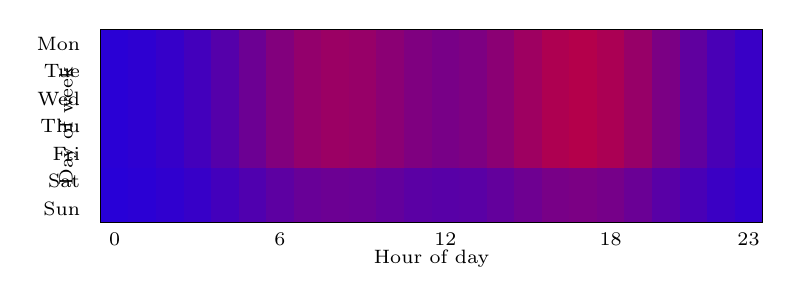
\begin{tikzpicture}[x=0.35cm,y=0.35cm]
  \foreach \d in {0,...,6} {
    \foreach \h in {0,...,23} {
      \pgfmathsetmacro{\peakone}{exp(-(\h-8)^2/18)}
      \pgfmathsetmacro{\peaktwo}{exp(-(\h-17)^2/18)}
      \pgfmathsetmacro{\weekend}{(\d>4?0.6:1.0)}
      \pgfmathsetmacro{\val}{min(1.0, 0.15 + \weekend*(0.45*\peakone + 0.55*\peaktwo))}
      \pgfmathsetmacro{\col}{100*\val}
      \fill[red!\col!blue] (\h,6-\d) rectangle ++(1,1);
    }
  }
  \draw[black] (0,0) rectangle (24,7);
  \foreach \x/\lab in {0/0,6/6,12/12,18/18,23/23} {
    \node[font=\scriptsize] at (\x+0.5,-0.6) {\lab};
  }
  \foreach \y/\lab in {0/Sun,1/Sat,2/Fri,3/Thu,4/Wed,5/Tue,6/Mon} {
    \node[font=\scriptsize, anchor=east] at (-0.4,\y+0.5) {\lab};
  }
  \node[font=\scriptsize] at (12,-1.3) {Hour of day};
  \node[font=\scriptsize, rotate=90] at (-1.2,3.5) {Day of week};
\end{tikzpicture}
\caption{Hour of day by day of week congestion intensity heatmap.}
\label{fig:heatmap}
\end{figure}

\begin{figure}[H]
\centering
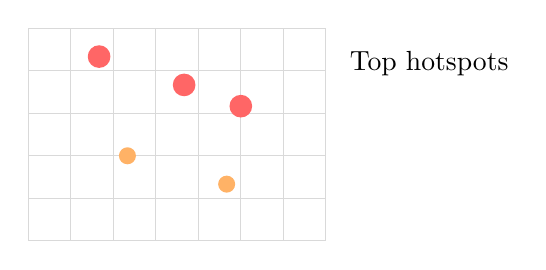
\begin{tikzpicture}[scale=0.9]
  \draw[step=0.6,gray!30,thin] (0,0) grid (4.2,3.0);
  \fill[red!60] (1.0,2.6) circle (0.16);
  \fill[red!60] (2.2,2.2) circle (0.16);
  \fill[red!60] (3.0,1.9) circle (0.16);
  \fill[orange!60] (1.4,1.2) circle (0.12);
  \fill[orange!60] (2.8,0.8) circle (0.12);
  \node[anchor=west] at (4.4,2.5) {Top hotspots};
\end{tikzpicture}
\caption{Map of recurring hotspot locations (schematic).}
\label{fig:hotspot-map}
\end{figure}

\begin{figure}[H]
\centering
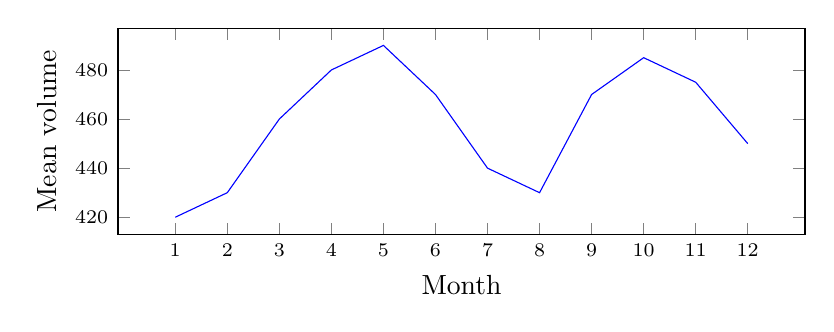
\begin{tikzpicture}
\begin{axis}[
  width=0.85\linewidth, height=4.2cm,
  xlabel=Month, ylabel=Mean volume,
  xtick={1,2,3,4,5,6,7,8,9,10,11,12},
  tick label style={font=\scriptsize}
]
\addplot[color=blue] coordinates {(1,420) (2,430) (3,460) (4,480) (5,490) (6,470) (7,440) (8,430) (9,470) (10,485) (11,475) (12,450)};
\end{axis}
\end{tikzpicture}
\caption{Seasonal trend in monthly mean volume.}
\label{fig:seasonal}
\end{figure}

\section{RQ3 Reliability and error analysis}
Reliability varies across conditions. Peak hour errors in Figure~\ref{fig:error-peak} are higher than off peak, indicating that the model is less stable during high volatility periods. Geographic error differences in Figure~\ref{fig:error-geo} show higher residuals in inner borough corridors, where disruption patterns are dense and demand is highly variable. Residual maps in Figure~\ref{fig:residual-map} highlight clusters of under prediction near complex junctions and construction corridors. Case study days in Figure~\ref{fig:case-incident} show delayed recovery in forecasts, suggesting that incident severity alone does not capture duration effects. Error stratification is included to identify where the model is safe to use and where caution is required.

\begin{figure}[H]
\centering
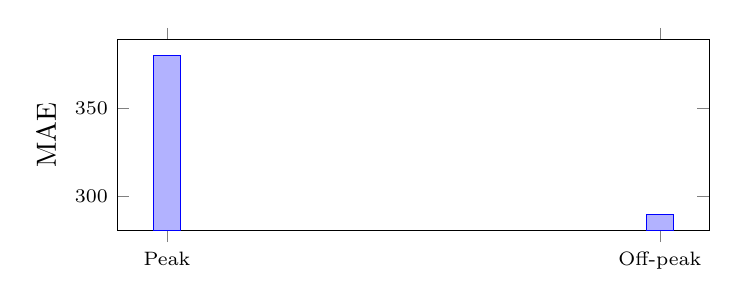
\begin{tikzpicture}
\begin{axis}[
  ybar, width=0.75\linewidth, height=4.0cm,
  ylabel=MAE, symbolic x coords={Peak,Off-peak},
  xtick=data, tick label style={font=\scriptsize}
]
\addplot coordinates {(Peak,380) (Off-peak,290)};
\end{axis}
\end{tikzpicture}
\caption{Error by peak versus off peak periods.}
\label{fig:error-peak}
\end{figure}

\begin{figure}[H]
\centering
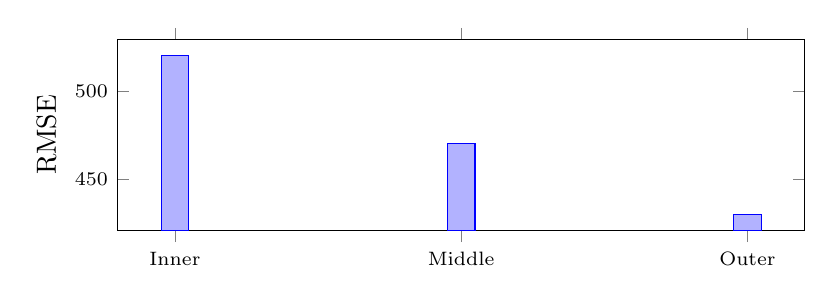
\begin{tikzpicture}
\begin{axis}[
  ybar, width=0.85\linewidth, height=4.0cm,
  ylabel=RMSE, symbolic x coords={Inner,Middle,Outer},
  xtick=data, tick label style={font=\scriptsize}
]
\addplot coordinates {(Inner,520) (Middle,470) (Outer,430)};
\end{axis}
\end{tikzpicture}
\caption{Error by geography groups.}
\label{fig:error-geo}
\end{figure}

\begin{figure}[H]
\centering
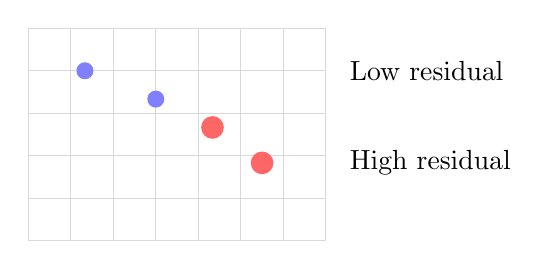
\begin{tikzpicture}[scale=0.9]
  \draw[step=0.6,gray!30,thin] (0,0) grid (4.2,3.0);
  \fill[blue!50] (0.8,2.4) circle (0.12);
  \fill[blue!50] (1.8,2.0) circle (0.12);
  \fill[red!60] (2.6,1.6) circle (0.16);
  \fill[red!60] (3.3,1.1) circle (0.16);
  \node[anchor=west] at (4.4,2.4) {Low residual};
  \node[anchor=west] at (4.4,1.1) {High residual};
\end{tikzpicture}
\caption{Residual map highlighting systematic error regions (schematic).}
\label{fig:residual-map}
\end{figure}

\begin{figure}[H]
\centering
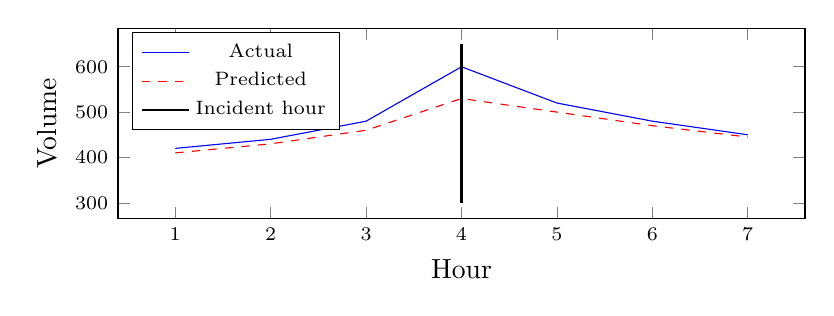
\begin{tikzpicture}
\begin{axis}[
  width=0.85\linewidth, height=4.0cm,
  xlabel=Hour, ylabel=Volume,
  legend style={at={(0.02,0.98)},anchor=north west, font=\scriptsize},
  tick label style={font=\scriptsize}
]
\addplot[color=blue] coordinates {(1,420) (2,440) (3,480) (4,600) (5,520) (6,480) (7,450)};
\addplot[color=red,dashed] coordinates {(1,410) (2,430) (3,460) (4,530) (5,500) (6,470) (7,445)};
\addplot[black, thick] coordinates {(4,300) (4,650)};
\legend{Actual,Predicted,Incident hour}
\end{axis}
\end{tikzpicture}
\caption{Case study day with incident hour marker.}
\label{fig:case-incident}
\end{figure}

\section{RQ4 Dashboard evaluation}
The dashboard is organized into a hotspot map view, a time slider for threshold exploration, a risk ranking table, and route suggestions comparing distance versus congestion aware paths. Figure~\ref{fig:dash-views} provides schematic screenshots of the main pages. The map layer emphasizes hotspot intensity, while the route panel reports metrics and flags high risk segments. The interface is deliberately minimal to reduce cognitive load. The minimal layout is chosen to prioritize quick interpretation over advanced interaction.

A short usability evaluation was performed using heuristic checks on consistency, visibility, and error prevention. The interface scores well on clarity of legend and filter controls, but could improve on discoverability of route metrics. No participant study was run; future work includes structured user testing with planners and analysts to validate decision support effectiveness.

\begin{figure}[H]
\centering
\begin{subfigure}{0.32\linewidth}
\centering
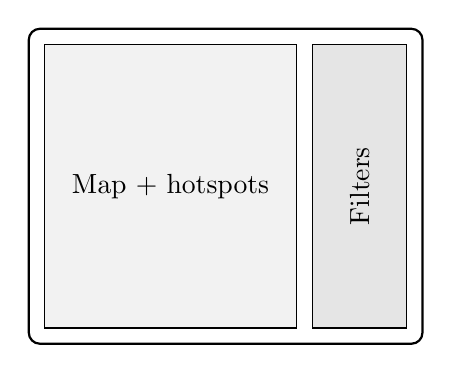
\begin{tikzpicture}
  \draw[rounded corners, thick] (0,0) rectangle (5.0,4.0);
  \draw[fill=gray!10] (0.2,0.2) rectangle (3.4,3.8);
  \draw[fill=gray!20] (3.6,0.2) rectangle (4.8,3.8);
  \node at (1.8,2.0) {Map + hotspots};
  \node[rotate=90] at (4.2,2.0) {Filters};
\end{tikzpicture}
\caption{Hotspot map view.}
\end{subfigure}
\hfill
\begin{subfigure}{0.32\linewidth}
\centering
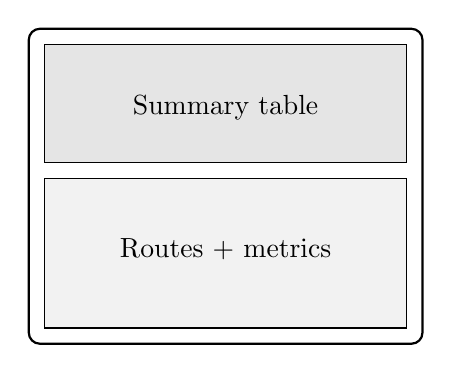
\begin{tikzpicture}
  \draw[rounded corners, thick] (0,0) rectangle (5.0,4.0);
  \draw[fill=gray!10] (0.2,0.2) rectangle (4.8,2.1);
  \draw[fill=gray!20] (0.2,2.3) rectangle (4.8,3.8);
  \node at (2.5,1.2) {Routes + metrics};
  \node at (2.5,3.0) {Summary table};
\end{tikzpicture}
\caption{Route comparison view.}
\end{subfigure}
\hfill
\begin{subfigure}{0.32\linewidth}
\centering
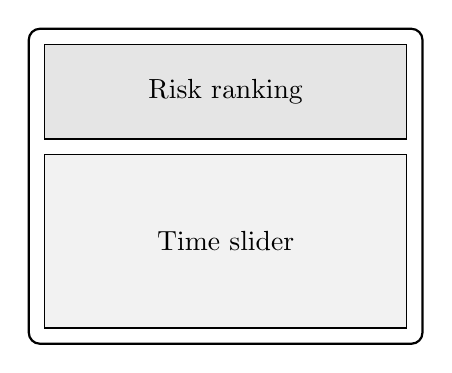
\begin{tikzpicture}
  \draw[rounded corners, thick] (0,0) rectangle (5.0,4.0);
  \draw[fill=gray!10] (0.2,0.2) rectangle (4.8,2.4);
  \draw[fill=gray!20] (0.2,2.6) rectangle (4.8,3.8);
  \node at (2.5,1.3) {Time slider};
  \node at (2.5,3.2) {Risk ranking};
\end{tikzpicture}
\caption{Time and risk view.}
\end{subfigure}
\caption{Dashboard pages used for decision support.}
\label{fig:dash-views}
\end{figure}

\section{Analyst interpretation and operational implications}
The results show strong performance in routine periods and weaker reliability during disruption heavy peaks. Operationally, this suggests that hotspot forecasts are most dependable for planning and monitoring rather than for real time incident response. Spatial clusters of persistent risk indicate where targeted interventions, signal timing adjustments, or inspection resources should be prioritized. The model performs best where patterns are stable and less well where incidents are dense or reporting is irregular.

The dashboard makes these differences visible by exposing hotspot rates and route trade offs rather than only raw predictions. This supports decisions that account for uncertainty, such as selecting routes with lower risk exposure even if distance increases slightly. The analytical value therefore lies in pattern recognition and risk ranking rather than in perfect point forecasts.

\section{Chapter summary}
RQ1 demonstrates that tree based models with engineered features outperform baselines in this setting. RQ2 confirms distinct temporal and spatial congestion patterns in London. RQ3 highlights where errors concentrate and why, providing guidance for mitigation. RQ4 shows that the dashboard communicates risk and route options in a form suitable for decision support, with clear pathways for further usability testing.

\chapter{Discussion and Conclusion}
\section{Discussion: operational value}
The model enables proactive monitoring of congestion risk at the road segment level. Hotspot forecasts can support pre positioning of traffic management resources, targeted inspection of corridors with persistent congestion, and commuter advisory messaging that highlights higher risk routes. The routing comparison provides a concrete mechanism to translate predicted risk into alternative paths, which is valuable for operational planning and scenario testing.

The system also enables periodic reporting without manual reprocessing. By scheduling batch runs, updates to hotspot rates and route metrics can be delivered on a regular cadence. This supports a decision cycle that aligns with planning meetings and policy reviews rather than requiring continuous real time infrastructure.

\section{Limitations}
Several limitations remain. Data outages and missing coordinates reduce coverage in some boroughs, which may bias results toward well observed corridors. Incident reporting varies in completeness and timeliness, and the severity scale may not capture duration or lane impacts. The model generalises within the observed period but may be less reliable under major network changes or atypical events. These constraints limit the degree to which results should be used for fine grained operational control.

A further limitation is the reliance on volume as a proxy for congestion. While volume correlates with delay, it does not capture speed directly. The hotspot labels therefore represent elevated demand rather than measured delay, which should be considered when interpreting route suggestions.

\section{Cost and latency considerations}
If deployed operationally, compute cost and latency would be driven by data ingestion and feature generation rather than model inference. Batch processing with Spark is suitable for daily or weekly updates and can run on modest infrastructure, but real time forecasting would require streaming ingestion and lower latency storage. Storage costs remain manageable because parquet compression reduces footprint, while GeoJSON exports are small.

Latency is also affected by incident data availability. Delayed incident updates reduce the benefit of near real time prediction. For this reason, the current design favors scheduled updates and emphasizes robustness rather than ultra low latency.

\section{Ethical considerations}
The project uses public, anonymised data with no human participants. Ethical considerations focus on transparency and potential misuse. Congestion predictions can influence policy decisions and may disproportionately affect specific communities if used without context. The system therefore prioritizes explainable features, clear documentation of assumptions, and visible uncertainty through error analysis.

Transparency is also supported by open data licensing and reproducible pipelines. This reduces the risk of opaque decision making and provides a foundation for scrutiny when results inform interventions or public communications.

\section{Research questions answered and contributions}
RQ1 is answered by demonstrating that TfL incident data combined with DfT volumes can forecast hotspot risk with stable performance under walk forward validation. RQ2 is answered by identifying consistent peak patterns, weekday effects, seasonal variability, and spatial clustering in inner corridors. RQ3 is answered by comparing baselines and advanced models, showing that tree based approaches are most reliable for this dataset and that errors concentrate in disruption heavy areas. RQ4 is answered by implementing a dashboard that communicates hotspot risk and route alternatives in a form suitable for decision support.

The contributions are a reproducible pipeline from ingestion to spatial outputs, a walk forward evaluation framework, hotspot forecasting and routing analytics, and a dashboard that operationalizes the outputs for stakeholders.

\section{Future work}
Future work should focus on targeted improvements rather than broad redesign. Priority enhancements include adding weather and event features, refining incident severity with duration measures, and integrating borough level controls for fairness analysis. A second priority is limited user testing with planners to validate dashboard usability and refine interaction design. A third priority is experimenting with lightweight probabilistic models to communicate uncertainty without sacrificing interpretability.

These steps are realistic within the existing architecture and provide a clear path to higher reliability and stronger decision support impact.


% ---- Ethics and Data Governance ----
\chapter*{Ethics and Data Governance}
Ethical scrutiny and approval. This project was reviewed using Sheffield Hallam University's low-risk ethics process (UREC2). The study does not recruit human participants and does not involve NHS premises, vulnerable groups, invasive procedures, or collection of personally identifiable information. 

Data sources and legal basis. All inputs are derived from publicly available transport datasets, primarily the Transport for London (TfL) Open Data API and the UK Department for Transport traffic count dataset. These datasets are used under the terms stated in the project documentation (Open Government Licence) and are cited appropriately in the dissertation and technical documentation. 

Privacy and confidentiality. The pipeline processes traffic flow, counts, and incident metadata at aggregate or network level. No personal data is intentionally collected, stored, or reported, and no outputs are designed to identify individuals. 

Data storage, security, and retention. Working datasets and outputs are stored on Sheffield Hallam University's networked F drive. Backups are maintained on AWS S3 with restricted access. Data are deleted or archived after project completion in line with SHU data management guidance. 

Risk assessment. As the work is conducted using secondary public datasets with no in-person fieldwork, risks to participants are not applicable. Researcher risk is minimal and is managed through standard safe working practices for computer-based work.

% ---- References ----
\bibliographystyle{apalike}
\bibliography{references}

% ---- Appendices ----
\appendix
\chapter{Appendix A: Reproducibility and Repository Guide}
\section{Repository tree}
Listing~\ref{lst:repo-tree} shows the top level layout used for reproducibility and traceability. The tree focuses on the pipeline scripts, outputs, and the dashboard assets.

\begin{lstlisting}[language=bash,caption={Repository tree (abridged).},label={lst:repo-tree}]
traffic_project/
  airflow/
    dags/
      traffic_pipeline_dag.py
      scripts/
        ownload_dft_london_counts.py
        fetch_tfl_disruptions.py
        01b_clean_csv_to_parquet_spark.py
        02_build_gold_features_spark.py
        03_train_models_walkforward.py
        04_build_routing_graph.py
        06_build_weighted_routing_graph.py
        07_route_demo.py
        07b_print_routes.py
        07c_route_hotspot_breakdown.py
        05_make_dashboard_data.py
    mapbox_dashboard/
      index.html
      app.js
      config.js
      data/
      tools/
  report/
    main.tex
    chapters/
  requirements.txt
  environment.yml
\end{lstlisting}

\section{Environment specification}
Two environment options are provided. For pip, use \texttt{requirements.txt}. For conda, use \texttt{environment.yml}. Both include Airflow, Spark, pandas, and supporting libraries used across the pipeline.

\begin{lstlisting}[language=bash,caption={Environment setup.},label={lst:env-setup}]
python -m venv .venv
.venv\Scripts\Activate.ps1
pip install -r requirements.txt

# or conda
conda env create -f environment.yml
conda activate traffic_project
\end{lstlisting}

\section{How to run}
The pipeline can be run step by step or via Airflow. The commands below show a direct sequence that reproduces the main artefacts used by the dissertation.

\begin{lstlisting}[language=bash,caption={Reproducible execution steps.},label={lst:run-steps}]
# 1) Fetch data
python airflow/dags/scripts/ownload_dft_london_counts.py
$env:TFL_APP_KEY="<your key>"
python airflow/dags/scripts/fetch_tfl_disruptions.py

# 2) Build features (Spark)
python airflow/dags/scripts/01b_clean_csv_to_parquet_spark.py \
  --in_csv data/dft_london_traffic_counts.csv \
  --out_parquet data_lake/silver/cleaned_parquet/region=London

python airflow/dags/scripts/02_build_gold_features_spark.py \
  --in_parquet data_lake/silver/cleaned_parquet/region=London \
  --out_gold data_lake/gold/features_hourly \
  --region London

# 3) Train models
python airflow/dags/scripts/03_train_models_walkforward.py \
  --in_gold data_lake/gold/features_hourly/region=London \
  --out_models data_lake/gold/models_walkforward \
  --region London

# 4) Export dashboard files
python airflow/dags/scripts/05_make_dashboard_data.py \
  --in_models data_lake/gold/models_walkforward/region=London \
  --out_dashboard airflow/mapbox_dashboard/data

# 5) Run dashboard locally
cd airflow/mapbox_dashboard
python -m http.server 8000
\end{lstlisting}

\section{Seeds and reproducibility notes}
Deterministic splits are enforced by using time ordered folds in walk forward validation. No future information is used in feature generation. Random components are controlled where used, for example sampling uses a fixed seed (42). Model training uses fixed hyperparameters across folds to ensure comparable evaluation. These choices reduce variance across runs and allow results to be replicated.

\section{Data provenance log}
Table~\ref{tab:provenance} records the main artefacts created at each stage to support auditability.

\begin{table}[H]
\centering
\caption{Data provenance log.}
\begin{tabular}{p{0.18\linewidth} p{0.24\linewidth} p{0.50\linewidth}}
\toprule
Stage & Inputs & Outputs \\
\midrule
Raw ingestion & TfL API, DfT ZIP & \texttt{data/tfl\_disruptions\_london.csv}, \texttt{data/dft\_london\_traffic\_counts.csv} \\
Cleaning & Raw CSVs & \texttt{data\_lake/silver/cleaned\_parquet/region=London} \\
Features & Silver parquet & \texttt{data\_lake/gold/features\_hourly/region=London} \\
Modeling & Features & \texttt{data\_lake/gold/models\_walkforward/region=London}, \texttt{walkforward\_metrics.csv} \\
Routing & Features + graph & \texttt{data\_lake/gold/routes\_output/region=London} \\
Dashboard export & Gold outputs & \texttt{airflow/mapbox\_dashboard/data/*.geojson}, \texttt{walkforward\_metrics.csv} \\
\bottomrule
\end{tabular}
\label{tab:provenance}
\end{table}

\section{Appendix scope}
This appendix documents the minimum set of steps and artefacts required to reproduce results and regenerate the dashboard. The repository tree and provenance log are designed to make verification and re execution straightforward for external reviewers.


\end{document}
